\appendix

\chapter{Chuỗi cử chỉ}
% \label{Appendix1}

\section{Sự thay đổi của $\sqrt{\beta}$ và $\sqrt{1-\beta}$}

Praesent in sapien. Lorem ipsum dolor sit amet, consectetuer 
adipiscing elit. Duis fringilla tristique neque. Sed interdum 
libero ut metus. Pellentesque placerat.


\begin{wrapfigure}{l}{0.3\textwidth}
	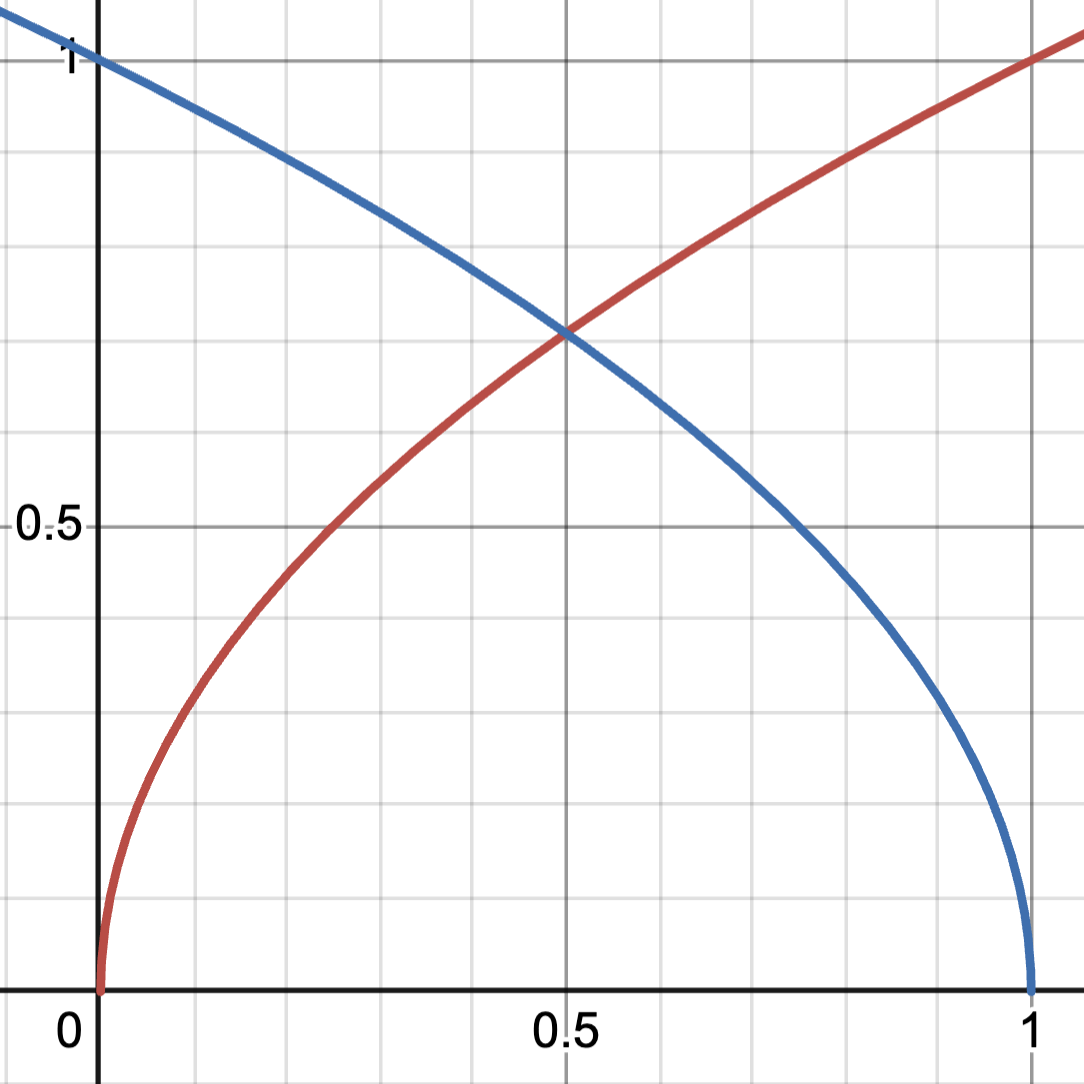
\includegraphics[width=0.9\linewidth]{images/beta_sqrtbeta}
	\label{fig:wrapfig}
\end{wrapfigure}

Praesent in sapien. Lorem ipsum dolor sit amet, consectetuer 
adipiscing elit. Duis fringilla tristique neque. Sed interdum

%\begin{figure*}[p]
%	\centering
%	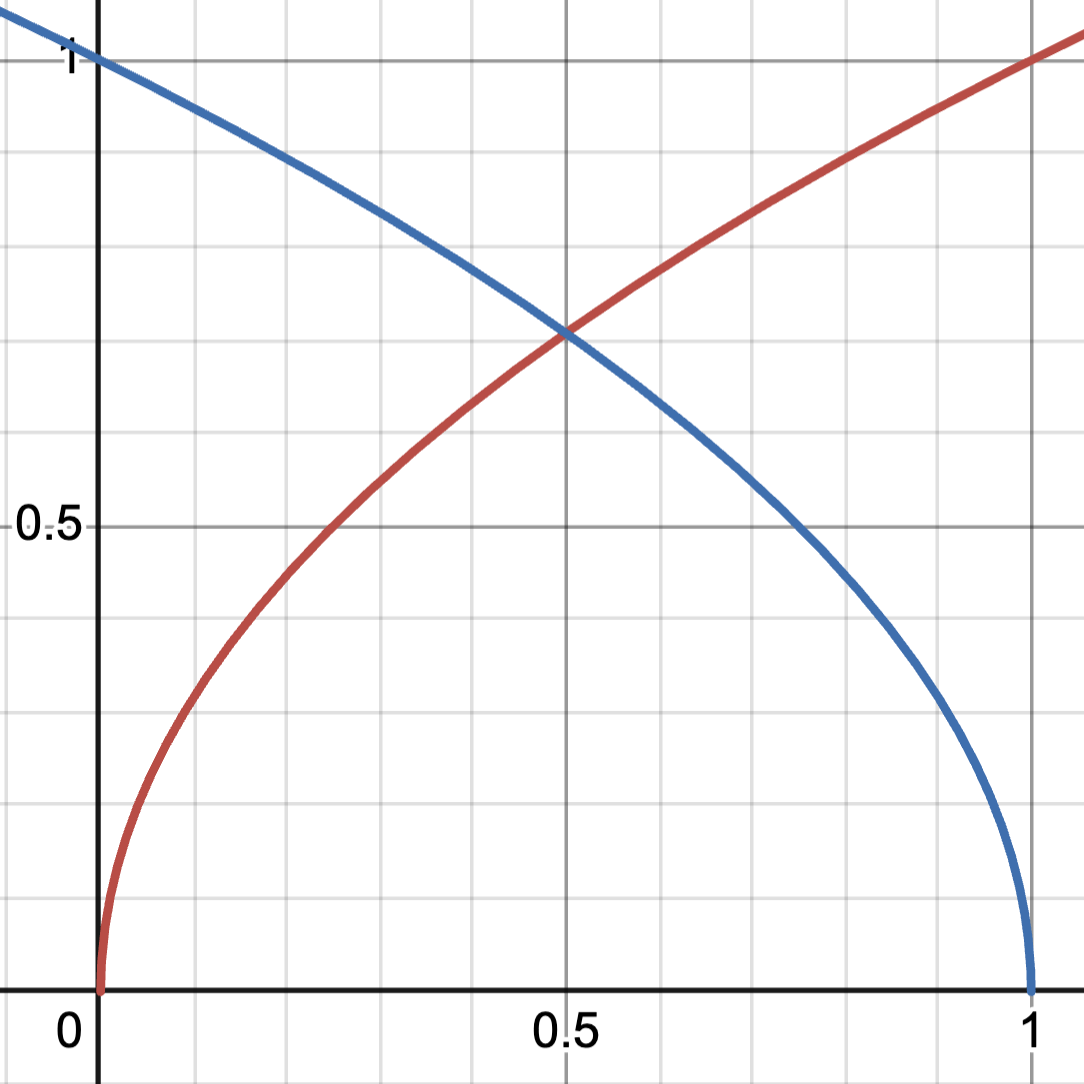
\includegraphics[width=0.5\linewidth]{images/beta_sqrtbeta}
%	\caption{Sự thay đổi của $\sqrt{\beta}$ và $\sqrt{1-\beta}$}
%	\label{fig:beta_sqrtbeta}
%\end{figure*}


You can put more than one value in the parameter, for instance, if you write [ht] LaTeX will try to position the figure here, but if it's not possible (the space may be insufficient) then the figure will appear at the top of the page. It is recommended to use more than one positioning parameter to prevent unexpected results.
